\section{Исследовательская часть}

\par В данном разделе проводится оценка результатов обработки потоковых аудиоданных с помощью разработанного программного комплекса.
Исследуется зависимость времени обработки аудиоданных, количества выделенной оперативной памяти для их обработки и вычислетельной нагрузки ЦПУ мобильного устройства, 
от наличия буферизации компонентом управления потоком данных.
Сравнивается количество выделенной оперативной памяти и затраченного времени для обработки аудиоданных с существующими аналогами.

\subsection{Исследование влияния буферизации компонентом управления потоком данных}
    \par В конструкторской части было рассмотрено, 
    что при периодическом сетевом подлючении критическая нагрузка ЦПУ может достигать $90-100\%$.
    Для решения данной проблемы был выделен компонент управления потоком данных, 
    который фильтрует и буферизует сетевые пакеты данных. 
    Также должно снизиться количество выделяемой оперативной памяти и время для обработки аудиопакетов.
    Чтобы потвердить данное утверждение необходимо провести соответствующий эксперимент.

    \par Получение объёма выделенной памяти, времени обработки данных и вычислительной нагрузки ЦПУ производилось с помощью Xcode Report Debuger.
    Для каждой из вышеперечисленных характеристик было произведено 10 замеров и взято среднее значение.
    Замеры проводились с использованием компонента управления потоком данных и без его участия.
    
    \par Для потоковой передачи аудиоданных был выбран аудиофайл со следующими характеристиками:
    \begin{itemize}
        \item[---] MP3 формат аудиофайла;
        \item[---] продолжительность аудио 14400 сек.;
        \item[---] разрешение звука 16 бит;
        \item[---] частота дискретизации 48 кГц;
    \end{itemize}

    \par На рис. \ref{fig:ram-throttler} представлено сравнение объёма выделенной оперативной памяти
    при потоковом получении аудиоданных с использованием компонента \newline управления потоком данных и без его участия.

    \begin{figure}[!h]
        \center{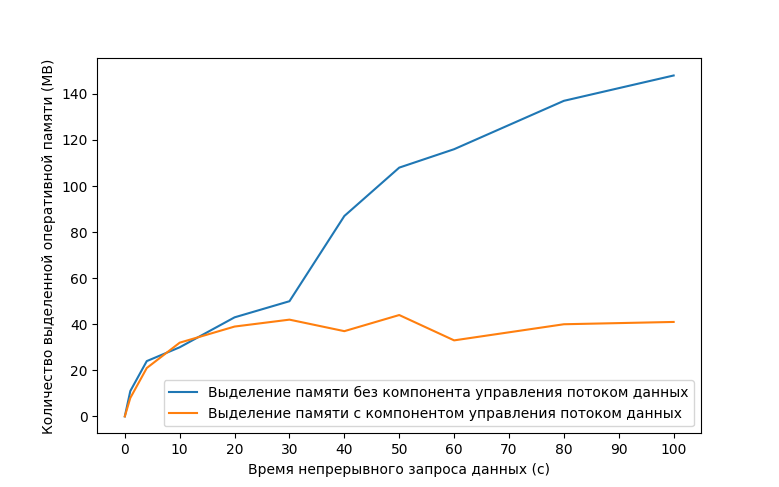
\includegraphics[scale=0.9]{img/ram-throttler.png}}
        \caption{
            Cравнение объёма выделенной оперативной памяти
            при потоковом получении аудиоданных 
            с использованием компонента управления потоком данных и без его участия.
        }
        \label{fig:ram-throttler}
    \end{figure}

    \par На графике видно, что зависимость выделения оперативной памяти для обработки аудиоданных от времени 
    без использования компонента управления потоком данных
    при периодическом сетевом подключении неубывающая.
    При использовании буферизации и фильтрации компонента объём выделенной памяти не привышает $44$ Мб.
    Следует, что использование механизмов буферизации и фильтрации 
    значительно снижает объём аудиоданных в оперативной памяти мобильного устройства.  

    \par Для замеров времени обработки сетевых аудиоданных необходимо также замерять время нахождения (простоя)
    сетового пакета после его получения.
    На рис. \ref{fig:time-throttler} представлен график сравнения времени обработки сетевых аудиоданных
    с использованием компонента управления потоком данных и без его участия.

    \begin{figure}[!h]
        \center{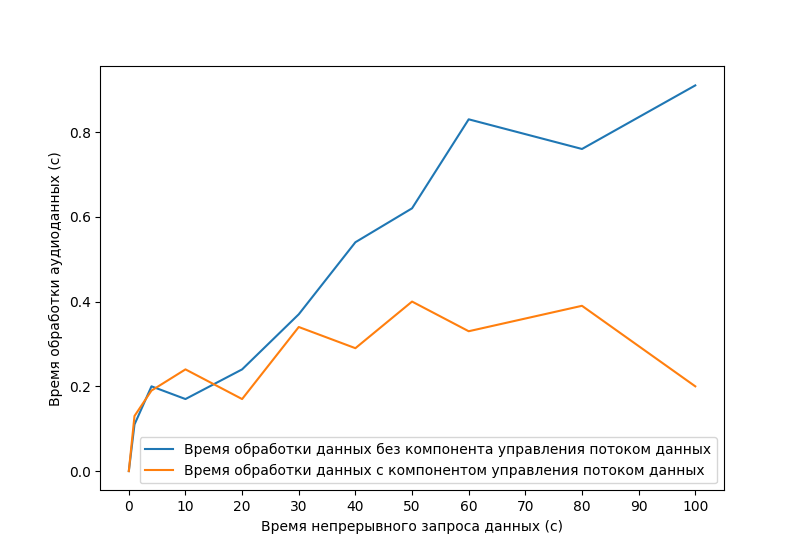
\includegraphics[scale=0.9]{img/time-throttler.png}}
        \caption{
            Сравнение времени обработки сетевых аудиоданных
            с использованием компонента управления потоком данных и без его участия.
        }
        \label{fig:time-throttler}
    \end{figure}

    \par Время обработки сетевых аудиоданных без использования компонента управления потоком возрастает.
    Это связано с простоем сетевых пакетов в очереде на обработку данных аудиосигнала.
    При использовании буферизации и фильтрации время обработки не превышает $0.4$ секунд.

    \par Для замеров нагрузки ЦПУ необходимо взять критическое значение (максимальную нагрузку) в процентах,
    которая потребляется мобильным приложением на операционной системе iOS, использующим разработанный программный комплекс.
    На рис. \ref{fig:cpu-throttler} представлен график сравнения максимальной нагрузки ЦПУ 
    с использованием компонента управления потоком данных и без его участия.
    \begin{figure}[!h]
        \center{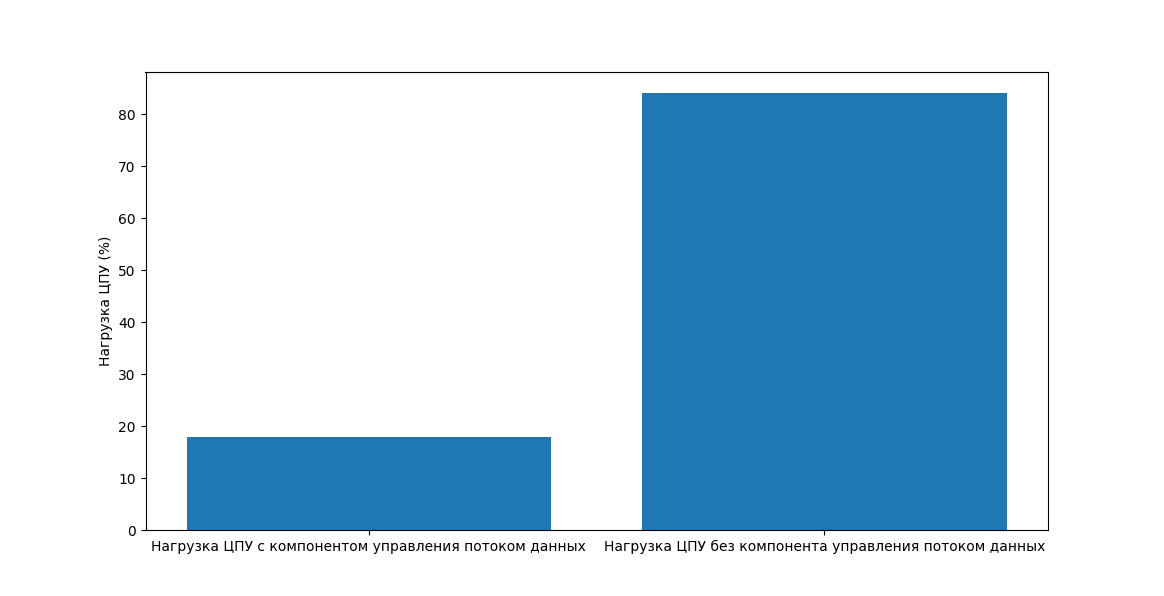
\includegraphics[scale=0.6]{img/throttler-cpu.png}}
        \caption{
            График сравнения максимальной нагрузки ЦПУ 
            с использованием компонента управления потоком данных и без его участия.
        }
        \label{fig:cpu-throttler}
    \end{figure}

    \par Из графика видно, что без использования буферизации и фильтрации максимальная нагрузка ЦПУ доходит до $84\%$.
    Использование компонента управления потоком данных позволило снизить максимальную нагрузку ЦПУ до $18\%$. 

    \par Опираясь на результаты проведённых замеров, можно сделать вывод, что с помощью компонента управления потоком данных удалось:
    \begin{itemize}
        \item[---] снизить нагрузку ЦПУ в $4.7$ раз;
        \item[---] избавиться от возрастающего времени обработки данных;
        \item[---] избавиться от возрастающей зависимости выделения оперативной памяти от времени;
        \item[---] ограничить время обработки данных и количество выделенной оперативной памяти до $44$ Мб и $0.4$ сек. соответсвенно;
    \end{itemize}

\subsection{Сравнение времени и выделения оперативной памяти для обработки данных с существующими аналогами}
    \par Произведён сравнительный анализ разработанного программного комплекса с существующими аналогами.
    В качестве аналогов были взяты: программный интерфейс AVAudioPlayer, программное обеспечение SwiftAudioPlayer.
    Данный выбор обусловлен следующими причинами:
    \begin{itemize}
        \item[---] поддержка воспроизведения потокового аудио;
        \item[---] полностью или частично использован комплекс программных итерфейсов AVFoundation;
        \item[---] поддержка разрешения звука 16 бит; 
    \end{itemize}
    
    \par В качестве сравниваемых характеристик были выбраны:
    \begin{itemize}
        \item[---] среднее время обработки аудиоданных;
        \item[---] среднее количество выделяемой оперативной памяти для обработки и воспроизведения аудиосигнала;
    \end{itemize}

    \par Для потоковой передачи аудиоданных был выбран аудиофайл со следующими характеристиками:
    \begin{itemize}
        \item[---] MP3 формат аудиофайла;
        \item[---] продолжительность аудио 360 сек.;
        \item[---] разрешение звука 16 бит;
        \item[---] частота дискретизации 48 кГц;
    \end{itemize}

    \par На рис. \ref{fig:disp-time} и \ref{fig:disp-ram} представлены графики сравнения среднего времени обработки аудиоданных 
    и среднее количество выделяемой оперативной памяти разработанного программного комплекса и вышеперечисленных аналогов.
    
    \par На основании графиков можно сделать вывод, 
    что среднее время обработки аудиоданных разработанного программного комплекса и AVAudioPlayer практически одинаково.
    Прирост времени при использовании AVAudioPlayer составляет $4\%$, что является незначительным.
    Среднее время обработки аудиоданных с помощью SwiftAudioPlayer больше, чем у разработанного программного комплекса на $20\%$.

    \par Разработанный программный комплекс имеет наименьшее потребление оперативной памяти для обработки сетевых аудиоданных.
    AVAudioPlayer выделяет на $14\%$ больше памяти, а SwiftAudioPlayer на $21\%$. Это связано с тем, 
    что они используют системный сегментатор аудиопакетов, 
    который хранит приходящие аудиопакеты даже после воспроизведения содержащегося в них аудиосигнала.

    \begin{figure}[!h]
        \center{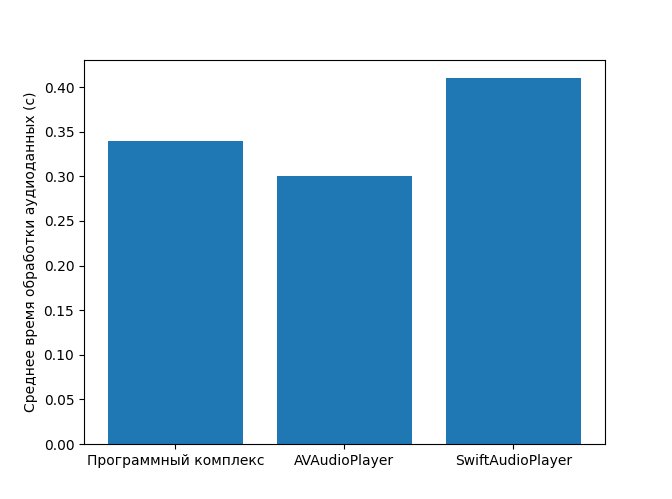
\includegraphics[scale=1.0]{img/sw-time.png}}
        \caption{
            График сравнения среднего времени обработки аудиоданных
            разработанного программного комплекса, AVAudioPlayer и SwiftAudioPlayer.
        }
        \label{fig:disp-time}
    \end{figure}

    \newpage

    \begin{figure}[!h]
        \center{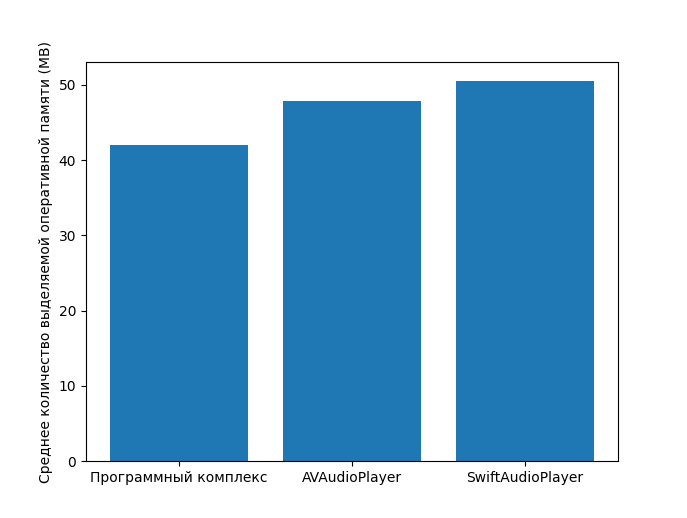
\includegraphics[scale=1.0]{img/sw-ram.png}}
        \caption{
            График сравнения среднего количества выделяемой оперативной памяти
            разработанного программного комплекса, AVAudioPlayer и SwiftAudioPlayer.
        }
        \label{fig:disp-ram}
    \end{figure}

\subsection*{Вывод}
    \par В данном разделе была произведена оценка результатов обработки потоковых аудиоданных с помощью разработанного программного комплекса.
    Исследовано влияние буферизации и фильтрации компонентом управления потоком данных на время обработки данных, количество выделяемой памяти, а также нагрузку ЦПУ.
    Был произведён сравнительный анализ разработанного программного комплекса с существующими аналогами.
    В результате исследований было установлено:
    \begin{itemize}
        \item[---] использование компонента управления потоком данных значительно снижает нагрузку ЦПУ, 
        время и количество выделенной оперативной памяти для обработки аудиоданных;
        \item[---] разработанный программный комплекс на $20\%$ быстрее обрабатывает аудиоданные, 
        чем SwiftAudioPlayer и на $4\%$ медленее, чем AVAudioPlayer;
        \item[---] разработанный программный потребляет меньшее количество оперативной памяти, чем его аналоги;
    \end{itemize}
\pagebreak